\documentclass[10pt,twocolumn,letterpaper]{article}

\usepackage{cvpr}
\usepackage{times}
\usepackage{epsfig}
\usepackage{graphicx}
\usepackage{amsmath}
\usepackage{amssymb}

\usepackage{color}
\usepackage{mathtools}
\usepackage{mathptmx}
\usepackage[11pt]{moresize}
\usepackage{wrapfig}
\usepackage{bbm}
\usepackage{xcolor}
\usepackage{tabularx}
\usepackage{bm}



\newcommand{\R}{\mathbb{R}}
\newcommand{\E}{\mathbb{E}}
\newcommand{\N}{\mathbb{N}}
\newcommand{\Z}{\mathbb{Z}}
\newcommand{\V}{\mathbb{V}}
\newcommand{\Q}{\mathbb{Q}}
\newcommand{\K}{\mathbb{K}}
\newcommand{\C}{\mathbb{C}}
\newcommand{\T}{\mathbb{T}}
\newcommand{\I}{\mathbb{I}}

% Include other packages here, before hyperref.

% If you comment hyperref and then uncomment it, you should delete
% egpaper.aux before re-running latex.  (Or just hit 'q' on the first latex
% run, let it finish, and you should be clear).
\usepackage[breaklinks=true,bookmarks=false]{hyperref}

\cvprfinalcopy % *** Uncomment this line for the final submission

\def\cvprPaperID{****} % *** Enter the CVPR Paper ID here
\def\httilde{\mbox{\tt\raisebox{-.5ex}{\symbol{126}}}}

% Pages are numbered in submission mode, and unnumbered in camera-ready
%\ifcvprfinal\pagestyle{empty}\fi
\setcounter{page}{1}
\begin{document}

%%%%%%%%% TITLE
\title{ On the Uncertainty of Wind Power Forecasts }  % \\  \small{Report}}

\author{Waleed  Alhaddad\\
King Abdullah University of Science (KAUST)\\
%4700 KAUST, Thuwal, Saudi Arabia\\
{\tt\small waleed.alhaddad@kaust.edu.sa}
% For a paper whose authors are all at the same institution,
% omit the following lines up until the closing ``}''.
% Additional authors and addresses can be added with ``\and'',
% just like the second author.
% To save space, use either the email address or home page, not both
\and
%Ra\'ul  Tempone\\
%KAUST/RWTH Aachen \\
% Templergraben 55, 52062 Aachen, Germany\\
%{\tt\small raul.tempone@kaust.edu.sa}
}

\maketitle
%\thispagestyle{empty}

%%%%%%%%% ABSTRACT

\begin{abstract}
Reliable wind power generation forecasting is crucial to meet energy demand, to trade and invest. We propose a model to simulate and quantify uncertainties in such forecasts. This model is based on Stochastic Differential Equations whose time-dependent parameters are inferred using continuous optimization of an approximate Likelihood function. The result is a skew stochastic process that simulates the uncertainty of wind power forecasts accounting for maximum power production limit and other temporal effects. We apply the model to historical Uruguayan data and forecasts.
\end{abstract}

%%%%%%%%% BODY TEXT
\section{Introduction}

    We propose a model to simulate and quantify uncertainties in wind power generation forecasts. This model is based on Stochastic Differential Equations (SDEs) whose time-dependent parameters are inferred using optimization techniques of an associated approximate Likelihood function. Through continuous optimization, we find the optimal parameters of an unbounded convex problem with convex constraints.

    We are able to simulate and quantify uncertainties in a variety of wind power generation forecasts while taking into account the skewness of the errors. This method is non-intrusive and is independent of forecasting technology or future developments. Through optimization, we update and tune the parameters of our SDE as we receive new sets of observations and their associated forecasts. Additionally, we are able to compare in a quantitative manner the different forecast technologies and how they behave in different real-world scenarios. This model is to be extended to the uncertainty quantification of other power generation sources such as the uncertainties in the power generation of solar power plants. This introduces new challenges in terms of optimization and modeling. Finally, we apply our model to synthetic and real wind power generation data for benchmarking. We apply the model to Uruguayan wind power production as determined by historical data and corresponding numerical forecasts for the year 2016-2017.

%-------------------------------------------------------------------------
\section{Model}


\subsection{Physical Model}

Let $X_t$ be the  wind power generation forecasts stochastic process defined by the  following parameterized stochastic differential equation (SDE), 
\begin{equation}
\begin{split}
dX_t &= a(X_t; \bm{\theta}) dt + b (X_t; \bm{\theta} ) dW_t \quad t > 0 \\
X_0 & = X_0
\end{split}\label{main}
\end{equation}


\begin{itemize}
%\item $\Delta_N$: any function of the number of samples, $N$. For example, $\Delta_N = \frac{1}{N}$.
\item $a(X_t; \bm{\theta})$: Drift function 
\item $b (X_t; \bm{\theta} )$: Diffusion function 
\item $\bm{\theta}$: a vector of parameters
\item $dW_t$: Standard Wiener random process.
\end{itemize}

%\subsection{Base Model}
%
%Let $V_t$ be the deviation of the wind power generation forecasts from  actual wind power generation. That is, $V_t$ models the errors or uncertainty of a given set of wind power generation forecasts. 
%
%We propose a forecast-error model based on the following parameterized stochastic differential equation (SDE), 
%\begin{equation}
%\begin{split}
%dV_t &= a(V_t; \bm{\theta}) dt + b (V_t; \bm{\theta} ) dW_t \quad t > 0 \\
%V_0 & = v_0
%\end{split}\label{main}
%\end{equation}
%
%
%\begin{itemize}
%%\item $\Delta_N$: any function of the number of samples, $N$. For example, $\Delta_N = \frac{1}{N}$.
%\item $a(V_t; \bm{\theta})$: Drift function 
%\item $b (V_t; \bm{\theta} )$: Diffusion function 
%\item $\bm{\theta}$: a vector of parameters
%\item $dW_t$: Standard Wiener random process.
%\end{itemize}


\subsection{Physical Restrictions}
It is necessary to keep  the power generation forecast plus its errors  inside the range $[0,1]$ after normalizing the power generated to the capacity of the power plant.  To ensure that, we choose our model to have zero diffusion near the boundaries. Hence, we  formulate the following diffusion  term, 
\begin{equation*}
\begin{split}
b(V_t; \bm{\theta}) &=  \sqrt{2 \theta \alpha p_t(1-p_t) X_t (1-X_t)}    \\
&= \sqrt{2 \theta \alpha p_t(1-p_t) (V_t +p_t ) (1-V_t-p_t)}  \\
\end{split}
\end{equation*}
It remains to control the drift term. As a first requirement, we need the drift term to be mean reverting to the power generation forecast. Thus, we formulate the following drift, 
\begin{equation}
a(V_t; \bm{\theta}) =  - \theta (X_t - p_t)
\end{equation}
However, this does not track the rate of change of the forecast $\dot{p}$ which  results in $X_t$ being out of sync with the forecast  as can be seen in Figure (\ref{sine_wave_shift})

\begin{figure}[t]
\begin{center}
%\fbox{\rule{0pt}{2in} \rule{0.9\linewidth}{0pt}}
   \includegraphics[width=0.8\linewidth]{conv_sine_shift.pdf}
\end{center}
   \caption{Example of the process $X_t$ following a sine wave without derivative tracking.}
\label{fig:long}
\label{fig:onecol}
\label{sine_wave_shift}
\end{figure}

For clarity of exposition, we switch to the point of view of the forecast prediction process $X_t = V_t + p_t$ and we include the derivative tracking in the base model,
\begin{equation}
\begin{split}
dX_t &= \hat{a}(X_t; \bm{\theta}) dt + \hat{b} (X_t; \bm{\theta} ) dW_t \quad t > 0 \\
X_0 & = x_0
\end{split}\label{main_X}
\end{equation}
where 
\begin{equation}
\begin{split}
\hat{a}(X_t; \bm{\theta}) &= \dot{p}_t + a(X_t; \bm{\theta}) =  \dot{p}_t - \theta \left(X_t - p_t\right)   \\
\hat{b}(X_t; \bm{\theta}) &=  b(X_t; \bm{\theta}) =  \sqrt{2 \theta \alpha p_t(1-p_t) X_t (1-X_t)}    \\
\end{split}
\end{equation}
Here the term $\dot{p}_t $ is not controlled to maintain that $X_t$ stays inside the range $[0,1]$. In other words, the zero drift line defined by  setting $\hat{a}(X_t; \bm{\theta}) =0$ must  be contained inside the range $[0,1]$. This line is given by   $ \frac{\dot{p}_t}{\theta}  + p_t $, we call it the line of zero drift or  the line of mean stationarity.
Thus, must have that, 
\begin{equation}
 0 \leq  \frac{\dot{p}_t}{\theta}  + p_t  \leq 1
\end{equation}
to keep the process $X_t$ inside the interval $[0,1]$.
The condition  can be rewritten as, 
\begin{equation}
\frac{- |\dot{p_t}|}{p_t} \leq \theta \leq \frac{|\dot{p}_t|}{1- p_t}
\end{equation}

To enforce the condition, we  define an adjusted drift $\theta = \theta_0 f( p_t, \dot{p}_t) $  which satisfies the condition when
\begin{equation}
\theta = \theta_0 f( p_t, \dot{p}_t) \leq \frac{|\dot{p}_t|}{\min (p_t, 1-p_t)} 
\end{equation}

Hence, we choose $\theta$ such that,
\begin{equation}
\theta = \max \left( \theta_0 \ , \ \frac{|\dot{p}_t|}{\min (p_t, 1-p_t)}  \right )
\end{equation}
\subsection{Model prescription }
We conclude that in order to respect the physical restrictions discussed above, we prescribe the following specifications and the final model becomes,
\begin{equation}
\begin{split}
dV_t &= a(V_t; \bm{\theta}) dt + b (V_t; \bm{\theta} ) dW_t \quad t > 0 \\
V_0 & = v_0
\end{split}\label{main}
\end{equation}

\begin{equation}
\begin{split}
a(V_t; \bm{\theta}) &= - \theta V_t \\
b(V_t; \bm{\theta}) &=\sqrt{2 \theta \alpha p_t(1-p_t) (V_t +p_t ) (1-V_t-p_t)}  \\
\end{split}
\end{equation}

with
\begin{equation}
\theta = \max \left( \theta_0 \ , \ \frac{|\dot{p}_t|}{\min (p_t, 1-p_t)}  \right )
\end{equation}

Where 
\begin{itemize}
\item $p_t$: Numerical wind power generation forecast.
\item $\theta >0$: Mean reversion parameter.
\item $\alpha>0$: Variability parameter.
\end{itemize}

The  SDE above defines the stochastic process $V_t$ which can be characterized by its transition denisity. Consider a set of M paths with N observations each, $ V^{M,N}=\{ V_{t_1^{M,N}} , V_{t_2^{M,N}} ,\ldots , V_{t_N^{M,N}} \}$ observed in intervals of $\Delta_N$. Then, the transitions of $V_t$ are given by the likelihood function,


\begin{equation}
\mathcal{L}(\theta;V) =\prod\limits_{j=1}^M \prod\limits_{i=1}^N \rho ( {V_{j,i+1}|V_{j,i}}, \bm{\theta})  \rho (V_{j,0}) 
\label{likelihood}
\end{equation}

The standard approach is approximating (\ref{likelihood}) by Gaussian transitions. However, this is inadequate in our case as we expect a skew symmetric stochastic process due to physical restrictions. Thus, we approximate the transitions by a Beta distribution. This is possible by matching the moments of the Beta distributions with the moments of the SDE defined above. The momoments are given by, 
\begin{equation}
\begin{split}
\E [V_t^k] &=  \E \Big[ \Big( \int a(V_t; \bm{\theta}_t) dt + \int b (V_t; \bm{\theta}_t ) dW_t \Big)^k \Big] \quad t > 0 \\
V_0 & = v_0
\end{split}\label{main_V_expectations}
\end{equation}
The above moments define a system of Ordinary Differential Equations,

\begin{equation}
\begin{split}
 \frac{dm_1(t)}{dt} &=    - \theta_t m_1(t)  \\
\frac{d m_{2}(t)}{dt}&= -2m_{2}(t) [\theta_t + \alpha_t \theta_t p_t(1-p_t) ] \\
&+ 2m_{1}(t)[\alpha_t \theta_t p_t (1-p_t) (1-2p_t)] \\
&+ 2\alpha_t \theta_t p_t^2(1-p_t)^2  \\
%m_2(0) = \E[V_0^2] = v_0^2\\
\end{split}
\end{equation}
With initial conditions,

\begin{equation}
\begin{cases}
&m_1(0)=\E[V_0]= v_0 \\
&m_2(0)=\E[V_0^2] = v_0^2 \\
\end{cases}
\end{equation}

where $m_1(t)$ and $m_2(t)$ are the first and second moments of the stochastic process $V_t$. As we are dealing with numerical wind power generation forecasts $p_t$, we do not have a closed form solution to this system of ODEs. Thus, this system is iteratively solved by means of numerical integration.

Once the moments $m_1(t)$ and $m_2(t)$ are obtained, we match them with the shape parameters of the Beta distribution. To allow for negative and positive values of the process $V_t$, we formulate a modified Beta distribution whose support is defined on $[a,b]=[-1,1]$.  We use the linear transformation $y= g(x)= a + (b-a) x $ and we obtain the probability density function,

\begin{equation}
\begin{split}
f_Y(y; \alpha , \beta )&= f_X(g^{-1}(y) ) \Big| \frac{\partial g^{-1}(y)}{\partial y }  \Big| \\
&= \frac{1}{B(\alpha, \beta) (b-a)} \Big(\frac{a-y}{b-a}\Big)^{\alpha -1}\Big(1-\frac{a-y}{b-a} \Big)^{\beta -1} \label{modified_Beta}
\end{split}
\end{equation}
where $B(\cdot,\cdot)$ is the Beta function. Also, we find that
\begin{equation}
\E[Y]= a + (b-a) \frac{\alpha}{\alpha + \beta}
\end{equation}
\begin{equation}
\V[Y]= (b-a)^2 \frac{\alpha \beta}{(\alpha + \beta)^2 (\alpha + \beta + 1)}
\end{equation}

And by matching the moments, we find that 

\begin{equation}
\alpha = \frac{(\tilde{\mu}_t-a) \left(\tilde{\mu}_t^2-\tilde{\mu}_t (a+b)+\tilde{\sigma}_t^2+a b\right)}{\tilde{\sigma}_t^2 (a-b)}
\end{equation}
\begin{equation}
\beta = \frac{(\tilde{\mu}_t-b) \left(\tilde{\mu}_t^2-\tilde{\mu}_t (a+b)+\tilde{\sigma}_t^2+a b\right)}{\tilde{\sigma}_t^2 (b-a)}
\end{equation}
where $\tilde{\mu}_t = m_1(t)$ and $\tilde{\sigma}_t^2= m_2(t)- m_1^2(t)$

\subsection{ Likelihood Optimization }

Combining the previous results and (\ref{likelihood}), we can express the log-likelihood function for $M$ paths,
\begin{equation}
\begin{split}
\ell(\alpha, \beta|V)&= \sum\limits_{j=1}^M \sum\limits_{i=1}^N (\alpha -1)\log \left(\frac{V_{j,i+1}+1}{2}\right)\\
& + (\beta -1) \log \left( 1-\frac{V_{j,i+1}+1}{2}\right) - \log \left( 2 B(\alpha, \beta)\right)\\ \label{Likelihood}
\end{split}
\end{equation} 

where $\alpha$ and $\beta$ are given by,

\begin{equation}
\alpha = - \frac{(1+\tilde{\mu}_t )(\tilde{\mu}_t^2 + \tilde{\sigma}_t^2 -1)}{2 \tilde{\sigma}_t^2} \quad \quad \beta =  \frac{(\tilde{\mu}_t-1 )(\tilde{\mu}_t^2 + \tilde{\sigma}_t^2 -1)}{2 \tilde{\sigma}_t^2} \label{param_transformed_beta}
\end{equation}

We will show that the log-likelihood function in (\ref{Likelihood}) is concave. Note that it is sufficient to check the log-likelihood of the standard Beta distribution for concavity since the modified Beta distribution log-likelihood is obtained through non-negative weighted summations and a linear transformation $g(x)$ in the given data that does not affect the parameters of interest. Thus, the concavity is preserved. 

We study the concavity of  log-likelihood of the standard Beta,
\begin{equation*}
\ell^*(\alpha, \beta |x)=-\log (B(\alpha ,\beta ))+(\alpha -1) \log (x)+(\beta -1) \log (1-x)\end{equation*}
It has been shown that the Beta function $B(\alpha, \beta)$ is log-concave in both its arguments on $(0, \infty)^2$ (see [1]) and the remaining terms are linear in $\alpha$ and $\beta$. Then, we conclude that the likelihood in (\ref{likelihood}) is indeed log-concave.\\

In order to infer the shape parameters $\alpha$ and $\beta$, we perform the following constrained maximuim likelihood optimization, 

\begin{equation}
(\alpha^* , \beta^*) = \arg \underset{\alpha>0, \beta>0}{\min} - \ell(\alpha, \beta | V^{M,N} )
\end{equation}
 
We solve the above optimization problem using L-BFGS to avoid full numerical computation of the Hessian matrix.


%which has a hessian of the form,
%\[ \mathcal{H}(\ell)=
%\left(
%\begin{array}{cc}
% \psi ^{(1)}(\alpha +\beta )-\psi ^{(1)}(\alpha ) & \psi ^{(1)}(\alpha +\beta ) \\
% \psi ^{(1)}(\alpha +\beta ) & \psi ^{(1)}(\alpha +\beta )-\psi ^{(1)}(\beta ) \\
%\end{array}
%\right) 
%\]
%where $\psi ^{(1)}$ is the trigamma function. $\mathcal{H}$'s determinant is given by,
%
%\begin{equation*}
%|\mathcal{H}| = \psi ^{(1)}(\alpha ) \psi ^{(1)}(\beta )-(\psi ^{(1)}(\alpha )+\psi ^{(1)}(\beta )) \psi ^{(1)}(\alpha +\beta )
%\end{equation*}
%For $\alpha>0$ and $\beta >0$, we have that the trigamma function $\psi ^{(1)}$ is strictly monotonically decreasing and that it satisfies the following inequality,
%\begin{equation}
%0<\frac{1}{x} \leq \psi ^{(1)}(x) \quad \text{for} \ \ x >0
%\end{equation}
%
%Then we have that, 
%\begin{equation}
% \frac{1}{\alpha\beta}<\psi ^{(1)}(\alpha ) \psi ^{(1)}(\beta ) 
%\end{equation}
%
%\begin{equation}
% \frac{1}{\alpha} \frac{1}{\alpha + \beta } <\psi ^{(1)}(\alpha ) \psi ^{(1)}(\alpha + \beta ) 
%\end{equation}
%
%\begin{equation}
% \psi ^{(1)}(\alpha ) \psi ^{(1)}(\beta ) > \psi ^{(1)}(\alpha ) \psi ^{(1)}(\alpha + \beta  ) \geq  \frac{1}{\alpha} \frac{1}{\alpha + \beta } 
%\end{equation}
%
%\begin{equation}
% \psi ^{(1)}(\alpha ) \psi ^{(1)}(\beta ) > \psi ^{(1)}(\beta ) \psi ^{(1)}(\alpha + \beta  ) \geq  \frac{1}{\alpha} \frac{1}{\alpha + \beta } 
%\end{equation}
%
%\begin{equation}
%\left(
%\begin{array}{c}
% -\psi ^{(1)}(\alpha ) \text{x1}^2-\text{x2}^2 \psi ^{(1)}(\beta )+(\text{x1}+\text{x2})^2 \psi ^{(1)}(\alpha
%   +\beta ) \\
%\end{array}
%\right)
%\end{equation}




\subsection{Data}
We apply the aforementioned method to Uruguayan Windpower Generation data and their corresponding numerical wind power production forecast. 

The wind power generation data set contains hourly samples of aggregated wind power production throughout the country. The samples are normalized according to the full installation power which varies across the data set. Each sample path contains 72 hourly observations and we have a total of 1217 sample paths spanning the year 2016 to 2017 (87,624 data points).

The numerical wind power generation forecast set contains  1217 forecasts of the wind power generation paths corresponding to the wind power generation data set mentioned above.


\begin{figure}[t]
\begin{center}
%\fbox{\rule{0pt}{2in} \rule{0.9\linewidth}{0pt}}
   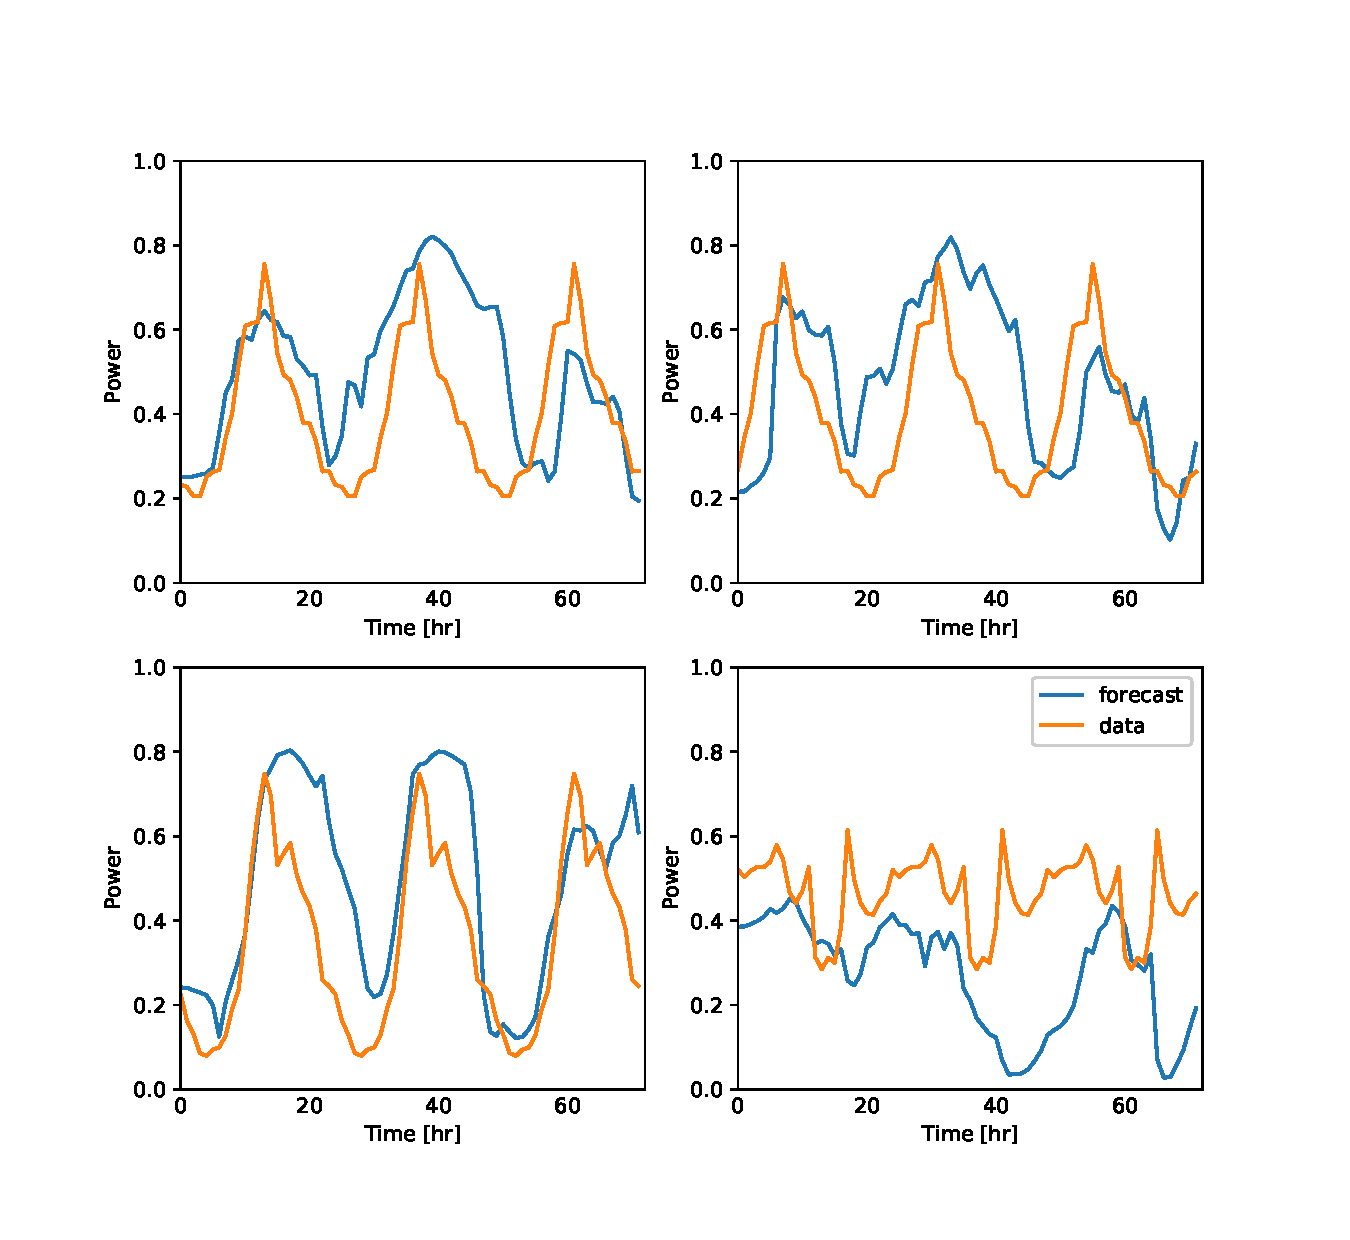
\includegraphics[width=0.8\linewidth]{forecast_data.eps}
\end{center}
   \caption{Examples of wind power generation from the data set along with the wind power generation forecast.}
\label{fig:long}
\label{fig:onecol}
\end{figure}





%-------------------------------------------------------------------------
\subsection{Results}
 We are able to obtain the parameters based on the complete data sets mentioned earlier. The parameters are given by $(\theta^*, \alpha^*)\approx (8,1)$. We show in Figure(\ref{fig:ISO}) the contours of the log-likelihood in $(\ref{Likelihood})$ using the full data set.
 
 
%We can also see in Figure() that the region surrounding the optimal parameters becomes more defined as we add more sample paths.
 
In Figure(\ref{fig:6hr}) and (\ref{fig:72hr}), we simulate sample forecast errors using the optimal parameters  $(\theta^*, \alpha^*)\approx (8,1)$ and obtain the associated confidence bands empirically using 10,000 sample paths for each forecast. Note that the confidence bands obtained are non-trivial and reflect the complexity of the uncertainties in the numerical wind power generation forecasts.

\begin{figure}[t]
\begin{center}
%\fbox{\rule{0pt}{2in} \rule{0.9\linewidth}{0pt}}
   \includegraphics[width=0.9\linewidth]{72hr_forecast_CI_343.pdf}
   \includegraphics[width=0.9\linewidth]{72hr_forecast_CI_573.pdf}
   \includegraphics[width=0.9\linewidth]{72hr_forecast_CI_396.pdf}

\end{center}
   \caption{ Examples of confidence bands obtained for the full 72 hour forecasts. }
\label{fig:72hr}
\end{figure}

\begin{figure}[t]
\begin{center}
%\fbox{\rule{0pt}{2in} \rule{0.9\linewidth}{0pt}}
   \includegraphics[width=0.9\linewidth]{6hr_forecast_CI_618.pdf}
   \includegraphics[width=0.9\linewidth]{6hr_forecast_CI_38.pdf}
   \includegraphics[width=0.9\linewidth]{6hr_forecast_CI_459.pdf}
\end{center}
   \caption{ Examples of confidence bands obtained for the first 6 hours of the forecasts. This is important as this specific forecasting company recomputes a new forecast every 6 hours.}
\label{fig:6hr}
\end{figure}



%\begin{figure}[t]
%\begin{center}
%%\fbox{\rule{0pt}{2in} \rule{0.9\linewidth}{0pt}}
%   \includegraphics[width=0.9\linewidth]{ISO_lines_detailed.pdf}
%   \includegraphics[width=0.9\linewidth]{ISO_lines_zoom_2.pdf}
%\end{center}
%   \caption{The Beta distribution log-likelihood evaluated given the complete data set of 1217 sample paths. The optimal parameter found are indicated by the blue dot.}
%\label{fig:ISO}
%\end{figure}






\begin{figure}[t]
\begin{center}
%\fbox{\rule{0pt}{2in} \rule{0.9\linewidth}{0pt}}
   \includegraphics[width=0.5\linewidth]{ellipse100_samples_dN=14e-02.pdf}
   \includegraphics[width=0.5\linewidth]{ellipse500_samples_dN=14e-02.pdf}
   \includegraphics[width=0.5\linewidth]{ellipse1193_samples_dN=14e-02.pdf}
\end{center}
   \caption{Shrinkage of the ellipse determined by the Hessian matrix of the log-likelihood around the point of optimality $(\theta, \alpha)\approx (8,1)$}
\label{ellipse_drawing}
\end{figure}
 
 
 \begin{figure}[t]
\begin{center}
%\fbox{\rule{0pt}{2in} \rule{0.9\linewidth}{0pt}}
   \includegraphics[width=0.5\linewidth]{ISO_100_samples_dN=14e-02.pdf}
   \includegraphics[width=0.5\linewidth]{ISO_500_samples_dN=14e-02.pdf}
   \includegraphics[width=0.5\linewidth]{ISO_1193_samples_dN=14e-02.pdf}
\end{center}
   \caption{Contour plot of the log-likelihood as more forecasts and data is added, point of optimality $(\theta, \alpha)\approx (8,1)$ indicated in black.}
\label{contour}
\end{figure}


\begin{figure}[t]
\begin{center}
%\fbox{\rule{0pt}{2in} \rule{0.9\linewidth}{0pt}}
   \includegraphics[width=0.5\linewidth]{Eigen_conv_samples_dN=14e-02.pdf}
   \includegraphics[width=0.5\linewidth]{ellipse_conv_samples_dN=14e-02.pdf}
\end{center}
   \caption{Convergence of the major and semi-axis of the ellipse  of the Hessian of the log-likelihood at the point optimality $(\theta, \alpha)\approx (8,1)$. Note that it is slightly faster than the expected rate of $1/\sqrt{M}$. This due to the fact that segments of some of the $M$ are uncorrelated, thus acting as an additional  uncorrelated sample to the rest of the path. }
\label{Ellipse_convergance}
\end{figure}
 
 
%\subsection{Discussion}




\subsection{Conclusion}

In this project, we have proposed a model to quantify the uncertainties in wind power generation forecasts. It is important to note that this approach is agnostic of forecasting technology. We have also taken into account the physical limits of the model by respecting the full installation power of the wind farm. Additionally, we have taken into account skew-symmetric errors for which the Beta distribution is an appropriate choice. The skewness of the forecast errors is necessary to correctly model the errors when operating near full installation power production or in cases of extremely low wind power production.

 



%-------------------------------------------------------------------------
\subsection{References}

\begin{itemize}
\item[][1] Dragomir, S., Agarwal, R., \& Barnett, N. (2000). Inequalities for Beta and Gamma functions via some classical and new integral inequalities. Journal of Inequalities and Applications, 2000(2), 504054. doi:10.1155/s1025583400000084
\end{itemize}




{\small
\bibliographystyle{ieee}
\bibliography{egbib}
}

\end{document}
